\documentclass{standalone}
\usepackage{pgfplots}

\begin{document}

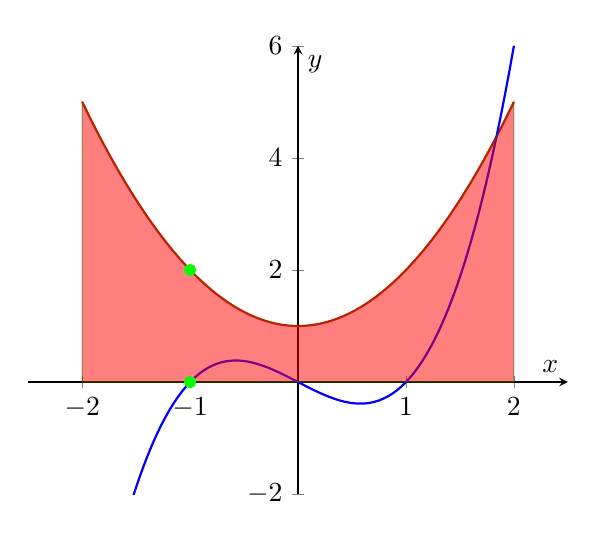
\begin{tikzpicture}
    \begin{axis}[
        axis lines = middle,
        xlabel = \(x\),
        ylabel = {\(y\)},
        ymin=-2, ymax=6,
        xmin=-2.5, xmax=2.5,
        samples=100,
        domain=-2:2,
        ]
        \addplot [red, thick] {x^2 + 1};
        \addplot [blue, thick] {x^3 - x};
        
        % Fill between the two curves from x=-2 to x=-1
        \addplot [green!50!black, fill=red, opacity=0.5] 
            {x^2 + 1} \closedcycle;
        
        % Mark points at x=-1
        \filldraw[green] (axis cs:-1,{(-1)^2+1}) circle (2pt);
        \filldraw[green] (axis cs:-1,{(-1)^3-(-1)}) circle (2pt);
    \end{axis}
\end{tikzpicture}

\end{document}